% Welcome! This is the unofficial University of Udine beamer template.

% See README.md for more informations about this template.

% This style has been developed following the "Manuale di Stile"
% (Style Manual) of the University of Udine. You can find the
% manual here: https://www.uniud.it/it/ateneo-uniud/ateneo-uniud/identita-visiva/manuali-immagine-stile/manuale-stile

% Note: for some reason, the RGB values specified in the manual
% do NOT render correctly in Beamer, so they have been redefined
% for this document using the high level chromo-optic deep neural
% quantistic technology offered by Microsoft Paint's color picker.

% We defined four theme colors: UniBrown, UniBlue, UniGold
% and UniOrange. For example, to write some uniud-brownish
% text, just use: \textcolor{UniBrown}{Hello!}

% Note that [usenames,dvipsnames] is MANDATORY due to compatibility
% issues between tikz and xcolor packages.

\documentclass[usenames,dvipsnames]{beamer}
\usepackage[utf8]{inputenc}
\usepackage{verbatim}
\usetheme{uniud}

% cleverref {{{
\usepackage[capitalize,nameinlink]{cleveref} % from https://tex.stackexchange.com/questions/187388/amsthm-with-shared-counters-messes-up-autoref-references
% }}}

\usepackage{graphicx}

%%% Bibliography {{{
\usepackage[style=authoryear,backend=biber]{biblatex}
\addbibresource{bibliography.bib}

% Author names in publication list are consistent
% i.e. name1 surname1, name2 surname2
% See https://tex.stackexchange.com/questions/106914/biblatex-does-not-reverse-the-first-and-last-names-of-the-second-author
\DeclareNameAlias{author}{first-last}
% }}}

%%% Suppress biblatex annoying warning {{{
\usepackage{silence}
\WarningFilter{biblatex}{Patching footnotes failed}
% }}}

%%% Some useful commands {{{
% pdf-friendly newline in links
\newcommand{\pdfnewline}{\texorpdfstring{\newline}{ }}
% Fill the vertical space in a slide (to put text at the bottom)
\newcommand{\framefill}{\vskip0pt plus 1filll}
% }}}


% \title[University of Udine Unofficial Beamer Theme]{Report: A formal approach for run-time verification of web applications using scope-extended LTL}
\title{Run-time verification of web applications}
% \date[May 1977]{May 25, 1977}
\author[Roberto Tonino]{
  Roberto Tonino
  \pdfnewline
  \texttt{tonino.roberto@spes.uniud.it}
}
\institute{\tiny Department of Mathematics, Computer Science and Physics, University of Udine}

% glossary {{{
\usepackage[acronym,automake]{glossaries}
\makeglossaries

% \newglossaryentry{WAUT}
% {
%     name=WAUT,
%     description={Web Application Under Test}
% }
\newacronym{waut}{WAUT}{Web Application Under Test}
% }}}


\begin{document}

\begin{frame}
\titlepage
\end{frame}

% \begin{frame}{Outline}
% \tableofcontents
% \end{frame}

% \section{Before you start}
% \begin{frame}{Overleaf users}

% \begin{alertblock}{Warning}
% You can ignore this slide if you're \textbf{not} working with Overleaf.
% \end{alertblock}

% \vskip 0.5cm

% Overleaf, Beamer and Biber do not always get along well together. For this reason, if you make a mistake while writing this presentation, in the drop-down error message you'll \textbf{always} get Biber-related error messages.

% \vskip 0.5cm

% Luckily, you just have to click on ``\texttt{go to first error/warning}'' and the UI will scroll to the line containing your mistake.

% \end{frame}

\section{Let's start from the end}
\begin{frame}{Let's start from the end}

  \begin{itemize}
    \item Tool for automatic verification of web applications
    \item Empirical results
    \item Limited setting in my opinion: no JavaScript
    \item Paper from 2013
  \end{itemize}
\end{frame}

\begin{frame}{Let's start from the end}
% \begin{figure}[h]
  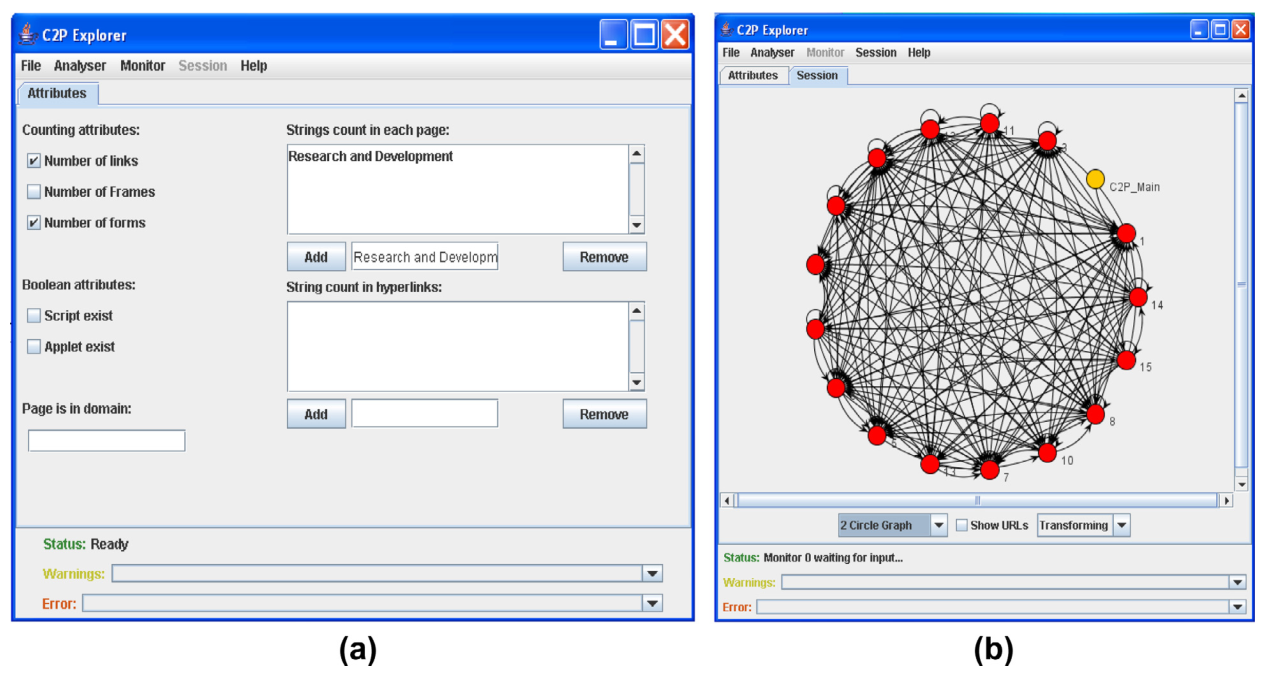
\includegraphics[width=\textwidth]{../img/screenshot_tool.png}
  % \caption{Example of a session automaton.}
  % \label{fig:example-session-automaton}
% \end{figure}
\end{frame}

\framecard{How?}

\section{How?}
\begin{frame}{How?}

  \begin{itemize}
    \item Communicating automata model
    \item LTL with a new operator
    \item Spin
  \end{itemize}
\end{frame}

\section{Single-display automata}
\begin{frame}{Single-display automata}
  \begin{itemize}
    \item Automata that represent a browser session of an user
    \item States are the pages of the session
    \item Transitions are clicks to links and form submissions
    \item Don't take into account other frames and/or windows
  \end{itemize}
\end{frame}

\section{Multi-display automata}
\begin{frame}{Multi-display automata}
  \begin{itemize}
    \item Automata that represent a browser session of an user
    \item Have links, form targets, frames
    \item Take into account multiple frames and/or browser windows
  \end{itemize}
\end{frame}


\end{document}

% vi: fdm=marker
